\documentclass[a4paper]{book}

\usepackage[pdftex]{graphicx}
\usepackage{wrapfig}

\newcommand{\HRule}{\rule{\linewidth}{0.5mm}}

\begin{document}

	\begin{titlepage}
	\begin{center}

	\textsc{\LARGE Hebrew University of Jerusalem}\\[1.5cm]
	
	\textsc{\Large Lectures Summary}\\[0.5cm]
	
	\HRule \\[0.4cm]
	{ \huge \bfseries Electricity and Magnetism (77102)}\\[0.4cm]
	
	\HRule \\[1.5cm]
	
	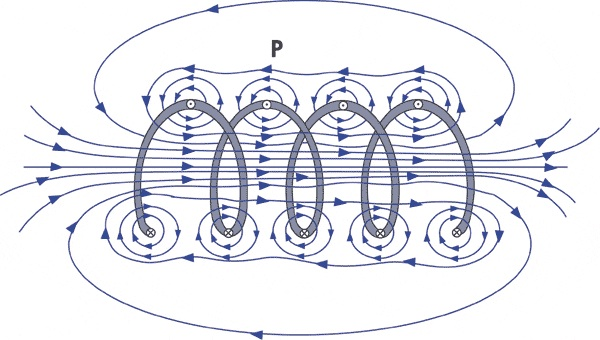
\includegraphics[scale=0.5]{coil1}~\\[1cm]
	
	\begin{minipage}{0.4\textwidth}
	\begin{flushleft} \large
	\emph{Author:}\\
	Avihu \textsc{Turzion}
	\end{flushleft}
	\end{minipage}
	\begin{minipage}{0.4\textwidth}
	\begin{flushright} \large
	\emph{Based on Lectures by:} \\
	Prof.~Hagai \textsc{Eizenberg}
	\end{flushright}
	\end{minipage}
	
	\vfill
	
	{\large \today}
	
	\end{center}
	
	\end{titlepage}
	
	\tableofcontents
	
	\chapter*{General Course Information}
	\addcontentsline{toc}{section}{General Course Information}
	
	\subsection*{Teacher Information}
	\addcontentsline{toc}{subsection}{Teacher Information}
	
	Prof.~\underline{\textsc{Hagai Eizenberg}} \\
	
	\begin{tabular}{r l}
	\textbf{Tel:} & 03-658-5228 \\
	\textbf{Office:} & Marx Building\\
	\end{tabular}
	
	\subsection*{Grade Structure}
	\addcontentsline{toc}{subsection}{Grade Structure}
	\begin{itemize}
		\item \%10 - Home assignments.
		\item \%20 - Midtest (only if greater than the final test grade). The midtest will occur between Electricity and Magnetism.
		\item \%70 - Final test or \%90 if greater than the midtest.
	\end{itemize}
	
	Possible bonuses: Each exercise is graded up to a 100, and a 100 is a single point to the final grade. There will be 13-14 exercises during the semester, so handing in all of the exercise helps improving the grade (assuming for some reason the final test was not a 100).
	
	\subsection*{Course 	Books}
	\addcontentsline{toc}{subsection}{Course Books}
	
	\begin{itemize}
		\item \textbf{Berkeley's Electricity and Magnetism by Edward M. Purcell} - Berkeley's Standard course book for Electricity and Magnetism.
		\item \textbf{Electricity and Magnetism by the Open University} - A direct translation of Berkeley's course book.
		\item \textbf{Classical Electrodynamics by J.D. Jackson} - A more rigorous book containing a lot of the rigorous mathematical proofs for the material. This is the standard course book for the more advanced course of Analytic Electricity.
	\end{itemize}
	
	\part{Electricity}
	\chapter{The Electric Charge}
	There are electric charges which are either positive or negative. Which is positive and which is negative is an arbitrary choice.
	
	\begin{wrapfigure}{r}{0.5\textwidth}
	\begin{center}
		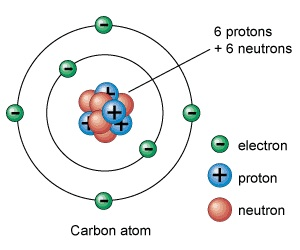
\includegraphics[scale=0.5]{carb-atom}
	\end{center}
	\caption{Carbon atom}
	\end{wrapfigure}
	
	Nowadays we have the model of the atom. We know that the electrons are negatively charged, the protons are positively charged and neutrons are not charged at all. Henceforth we'll discuss a charge by the amount of charge of a single electron marked as $q=e$. An amazing fact is that the proton is charged by the exact same amount of charge only in the opposite sign. The level of this accuracy is staggering, and if this balance would not have existed stable matter as we know it could not exist. The level of accuracy to which the charge of the protons and electrons was measured is $10^{-20}$.
	
	After an experiment in class we can conclude that same-signed charges repel each other, but different-signed charges attract each other.
	
	\subsection*{Conservation of Charge}
	
	Charge cannot be created out of thin air. In a closed system the charge must be preserved. This means that at the end of an operation the amount of charge in the system must be identical to before the start of the operation unless charge was inserted or taken to the outside.
	
	\subsection*{Charge Discreteness}
	
	A charge is discrete entity that its smallest quanta is the charge of an electron - \textbf{$e$}.
	
	\subsection*{Units}
	The course is taught using MKS units. The Open University and the Purcell and Jackson books work with CGS units.
	
	The name of the charge unit is: Coulomb. The charge of an electron expressed in Coulombs: $e = 1.602 \cdot 10^{-19}C$
	
	In CGS the charge is measured in 'esu' which is an abbreviation for 'electrostatic units'. The charge of an electron in these units: $e = 4.8 \cdot 10^{-10} esu$
	
	As opposed to Mechanics, the meaning of using a different set of units in Electricity and Magnetism is getting a different set of equation
	
	\section{Coulomb's Law}
	
	An inverse-square law that defines the force exerted by charged particles. The law must contain a linear dependence between the 2 charges in the system. The force is a vector and it's in the direction from the 1st charge to the 2nd charge.
	
	\begin{equation}
	\vec{F}_2 = \frac{q_1 q_2}{\vec{r}_{12}^2}\hat{r}_{12}
	\end{equation}
	
	\textbf{Unit vector in a direction of a certain vector:} $\hat{r} = \frac{\vec{r}}{|\vec{r}|}$
\end{document}